\documentclass[final,hyperref={pdfpagelabels=false}]{beamer}

\usepackage[T1]{fontenc}
\usefonttheme{professionalfonts}
\usepackage[sfmath,slantedGreeks]{kpfonts}
\usepackage[utf8]{inputenc}
\usepackage[orientation=portrait,size=a0,scale=1.4]{beamerposter}
\usepackage{graphicx,siunitx}

% \usetheme{Madrid}
\usecolortheme{beaver}
\setbeamertemplate{navigation symbols}{}

% Customise the caption: do not insert the caption name, nor the number, just
% insert a smaller caption text.
\setbeamertemplate{caption}{\scriptsize\insertcaption}

% % beaver è un tema grigio-rosso, ma non cambia il colore dei bullet di itemize e
% % di enumerate.  Il seguente comando serve a impostarli al colore darkred
% % definito nel tema beaver.
% \setbeamercolor{structure}{fg=darkred}

% \definecolor{darkblue}{rgb}{0,0,0.8}

%%%%%%%%%%%%%%%%%%%%%%%%%%%%%%%%%%%%%%%%%%%%%%%%%%%%%%%%%%%%%%%%%%%%%%%%%%%%%%%%
%%%%%%%%%%%%%%%%%%%%%%%%%%%%%%%%%%%%%%%%%%%%%%%%%%%%%%%%%%%%%%%%%%%%%%%%%%%%%%%%
%%%%%%%%%%%%%%%%%%%%%%%%%%%%%%%%%%%%%%%%%%%%%%%%%%%%%%%%%%%%%%%%%%%%%%%%%%%%%%%%

%% Colors

% Some tango colors
% butter (yellowish)
\definecolor{tabutter}{rgb}{0.98824, 0.91373, 0.30980}		% #fce94f

% orange
\definecolor{taorange}{rgb}{0.98824, 0.68627, 0.24314}		% #fcaf3e
\definecolor{ta2orange}{rgb}{0.96078, 0.47451, 0}		% #f57900

% Custom colors
\definecolor{mm3orange}{rgb}{0.90784, 0.36078, 0}
\definecolor{mmskyblue}{rgb}{0.34706, 0.56078, 0.81176}
\definecolor{mm2skyblue}{rgb}{0.10392, 0.39608, 0.64314}
\definecolor{mm3skyblue}{rgb}{0.02549, 0.29020, 0.52941}
\definecolor{mmLightSteelBlue}{rgb}{.5, .77, .87}

\selectcolormodel{cmyk}

\setbeamercolor{headline}{fg=tabutter,bg=mm3skyblue}
\setbeamercolor{footline}{fg=tabutter, bg=mm3skyblue}
\setbeamerfont{footline}{size=\large}
\setbeamercolor{separation line}{bg=ta2orange}
\setbeamercolor{title in headline}{fg=white}
\setbeamercolor{author in headline}{fg=white}
\setbeamercolor{institute in headline}{fg=white}

\setbeamercolor{framesubtitle}{fg=white, bg=ta2gray}
\setbeamercolor{author in head/foot}{fg=white, bg=mm3skyblue}
\setbeamercolor{title in head/foot}{fg=white, bg=black}

\setbeamercolor*{normal text}{fg=white, bg=mmLightSteelBlue}
\setbeamercolor*{block body}{bg=white,fg=black}
\setbeamercolor*{block title}{fg=white,bg=mm3skyblue}
\setbeamerfont{block title}{size=\large,series=\bf}
\setbeamercolor{upper separation line head}{fg=ta2orange}

\setbeamercolor*{example body}{fg=lightgray,bg=black}
\setbeamercolor*{example text}{fg=lightgray,bg=black}
\setbeamercolor*{example title}{bg=taorange,fg=ta2gray}

\setbeamercolor{alerted text}{fg=mm3orange}
\setbeamercolor{structure}{fg=mm2skyblue}

% adapt height of imtemize rectangles
\setbeamertemplate{itemize items}[circle]
% \setbeamertemplate{itemize item}{\raisebox{0.12ex}{$\blacktriangleright$}\hskip.1em}
% \setbeamertemplate{itemize subitem}{\raisebox{0.12ex}{$\triangleright$}\hskip.1em}
% or define your own template using \defbeamertemplate{itemize item}, see beameruserguide.pdf

% equal font sizes for all levels
\setbeamerfont{itemize/enumerate body}{size=\normalsize}
\setbeamerfont{itemize/enumerate subbody}{size=\normalsize}
\setbeamerfont{itemize/enumerate subsubbody}{size=\normalsize}

% Templates
% \setbeamertemplate{block begin}{
%   \vskip.75ex
%   \begin{beamercolorbox}[ht=3.5ex,dp=0.5ex,center,leftskip=-1em,colsep*=.75ex]{block title}%
%     \usebeamerfont*{block title}%
%     {\phantom{Gg}\insertblocktitle}% phantom because of baseline problem
%   \end{beamercolorbox}%
%   {\ifbeamercolorempty[bg]{block body}{}{\nointerlineskip\vskip-0.5pt}}%
%   \usebeamerfont{block body}%
%   \begin{beamercolorbox}[leftskip=1em,colsep*=.75ex,sep=0.5ex,vmode]{block body}%
%     \ifbeamercolorempty[bg]{block body}{\vskip-.25ex}{\vskip-.75ex}\vbox{}%
%   }
%   \setbeamertemplate{block end}{
%   \end{beamercolorbox}
% }

\setbeamertemplate{headline}{
  \leavevmode
  \begin{beamercolorbox}[wd=\paperwidth]{headline}
    \begin{columns}[T]
      \begin{column}{0.02\paperwidth}
      \end{column}
      \begin{column}{.12\paperwidth}
        \vskip4ex
        \begin{center}
          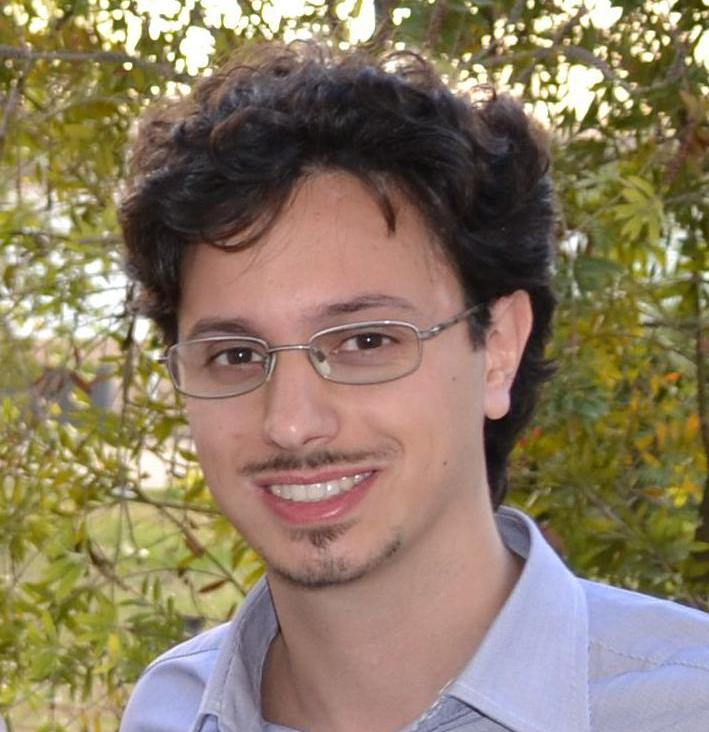
\includegraphics[width=0.94\columnwidth]{figures/giordano.jpg} \\[1.5ex]
          \href{mailto:Mose.Giordano@le.infn.it}{mose.giordano@le.infn.it}~
          \(\vcenter{\hbox{
\includegraphics[scale=1.3]{figures/mail}}}\)
        \end{center}
        \vskip2ex
      \end{column}
      \begin{column}{.7\paperwidth}
        \vskip4ex
        \begin{center}
          \usebeamercolor{title in
            headline}{\color{fg}\textbf{\Huge{\inserttitle}}\\[1.1ex]}
          \usebeamercolor{author in
            headline}{\color{fg}\Large{\insertauthor}\\[1.2ex]}
          \usebeamercolor{institute in
            headline}{\color{fg}\large{\insertinstitute}\\[1ex]}
        \end{center}
      \end{column}
      \begin{column}{.16\paperwidth}
        \vskip4ex
        \begin{center}
          
\includegraphics[width=.42\columnwidth]{figures/logo-unisalento.pdf} \qquad
          
\includegraphics[width=.42\columnwidth]{figures/infn.jpg} \\[2.8ex]
          
\includegraphics[width=.94\columnwidth]{figures/dipartimento.png}
        \end{center}
        \vskip2ex
      \end{column}
      \begin{column}{.02\paperwidth}
      \end{column}
    \end{columns}
    \vskip1ex
  \end{beamercolorbox}

  \begin{beamercolorbox}[wd=\paperwidth]{lower separation line head}
    \rule{0pt}{3pt}
  \end{beamercolorbox}
}

\setbeamertemplate{footline}{
  \begin{beamercolorbox}[wd=\paperwidth]{upper separation line foot}
    \rule{0pt}{3pt}
  \end{beamercolorbox}

  % \leavevmode%
  \begin{beamercolorbox}[ht=4ex,leftskip=1em,rightskip=1em]{author in head/foot}%
    Summer Course on Exoplanets
    \hfill
    La Palma, Canary Islands, \insertdate
    \vskip0.9ex
  \end{beamercolorbox}
  \vskip0pt%
  % \begin{beamercolorbox}[wd=\paperwidth]{lower separation line foot}
  %   \rule{0pt}{3pt}
  % \end{beamercolorbox}
}

%%%%%%%%%%%%%%%%%%%%%%%%%%%%%%%%%%%%%%%%%%%%%%%%%%%%%%%%%%%%%%%%%%%%%%%%%%%%%%%%
%%%%%%%%%%%%%%%%%%%%%%%%%%%%%%%%%%%%%%%%%%%%%%%%%%%%%%%%%%%%%%%%%%%%%%%%%%%%%%%%
%%%%%%%%%%%%%%%%%%%%%%%%%%%%%%%%%%%%%%%%%%%%%%%%%%%%%%%%%%%%%%%%%%%%%%%%%%%%%%%%


\newcommand{\arxiv}[1]{{\usebeamercolor[fg]{bibliography entry note}
    \href{http://arxiv.org/abs/#1}{arXiv: \texttt{#1}}}}
\newcommand{\doi}[1]{{\usebeamercolor[fg]{bibliography entry note}
    \href{http://dx.doi.org/#1}{\textsc{doi}: \texttt{#1}}}}

\DeclareMathOperator{\e}{\mathrm{e}}
\DeclareMathOperator{\uimm}{\mathrm{i}} % unità immaginaria
\renewcommand{\phi}{\varphi}
\renewcommand{\epsilon}{\varepsilon}
% complesso coniugato: \conjg{z}
\newcommand{\conjg}[1]{\overline{#1}}
\newcommand{\tah}[1]{\tilde{#1}}
% Nelle presentazioni il neretto non si distingue bene, ridefinisco \bm come \vec
\newcommand*{\dd}{\mathop{}\!\textup{d}} % Operatore differenziale \dd
% Derivata totale: \toder[ordine]{funzione}{variabile}
\newcommand*{\toder}[3][]{\frac{{\dd^{#1}}#2}{\dd {#3}^{#1}}}
\newcommand*{\ltoder}[3][]{{\dd^{#1}}#2/\dd {#3}^{#1}}

\newcommand{\advice}{
\includegraphics[height=0.8em]{figures/light-bulb}}
\newcommand{\warning}{
\includegraphics[height=0.6em]{figures/Warning-icon}}

\newcommand{\planeticon}[1]%
{\(\vcenter{\hbox{\includegraphics[height=1em]{figures/#1}}}\)}

\title{Estimating orbital period of exoplanets \\
  in microlensing events}
\author{\texorpdfstring{\textsc{Mosè Giordano}, \textsc{Achille A. Nucita},
    \textsc{Francesco De Paolis}, \textsc{Gabriele Ingrosso}}{Mosè Giordano,
    Achille A. Nucita, Francesco De Paolis, Gabriele Ingrosso}}
\institute[University of Salento and INFN Lecce]{Department of Mathematics and
  Physics ``\emph{E. De Giorgi}'', University of Salento, Lecce, Italy \\[0.8ex]
  INFN, Section of Lecce, Italy}
\date{24 September--2 October 2014}

\begin{document}
\begin{frame}
  \begin{columns}
    %%% Left column
    \begin{column}{0.44\columnwidth}
      \begin{minipage}[T]{\columnwidth}
        \begin{block}{Gravitational lensing\hfill \planeticon{mercury}}
          A \alert{gravitational lens} is a distribution of matter whose
          gravitational field distorts space-time, bends light rays and
          \alert{amplifies} the brightness of a source star coming to an
          observer
          \begin{figure}
            \centering
            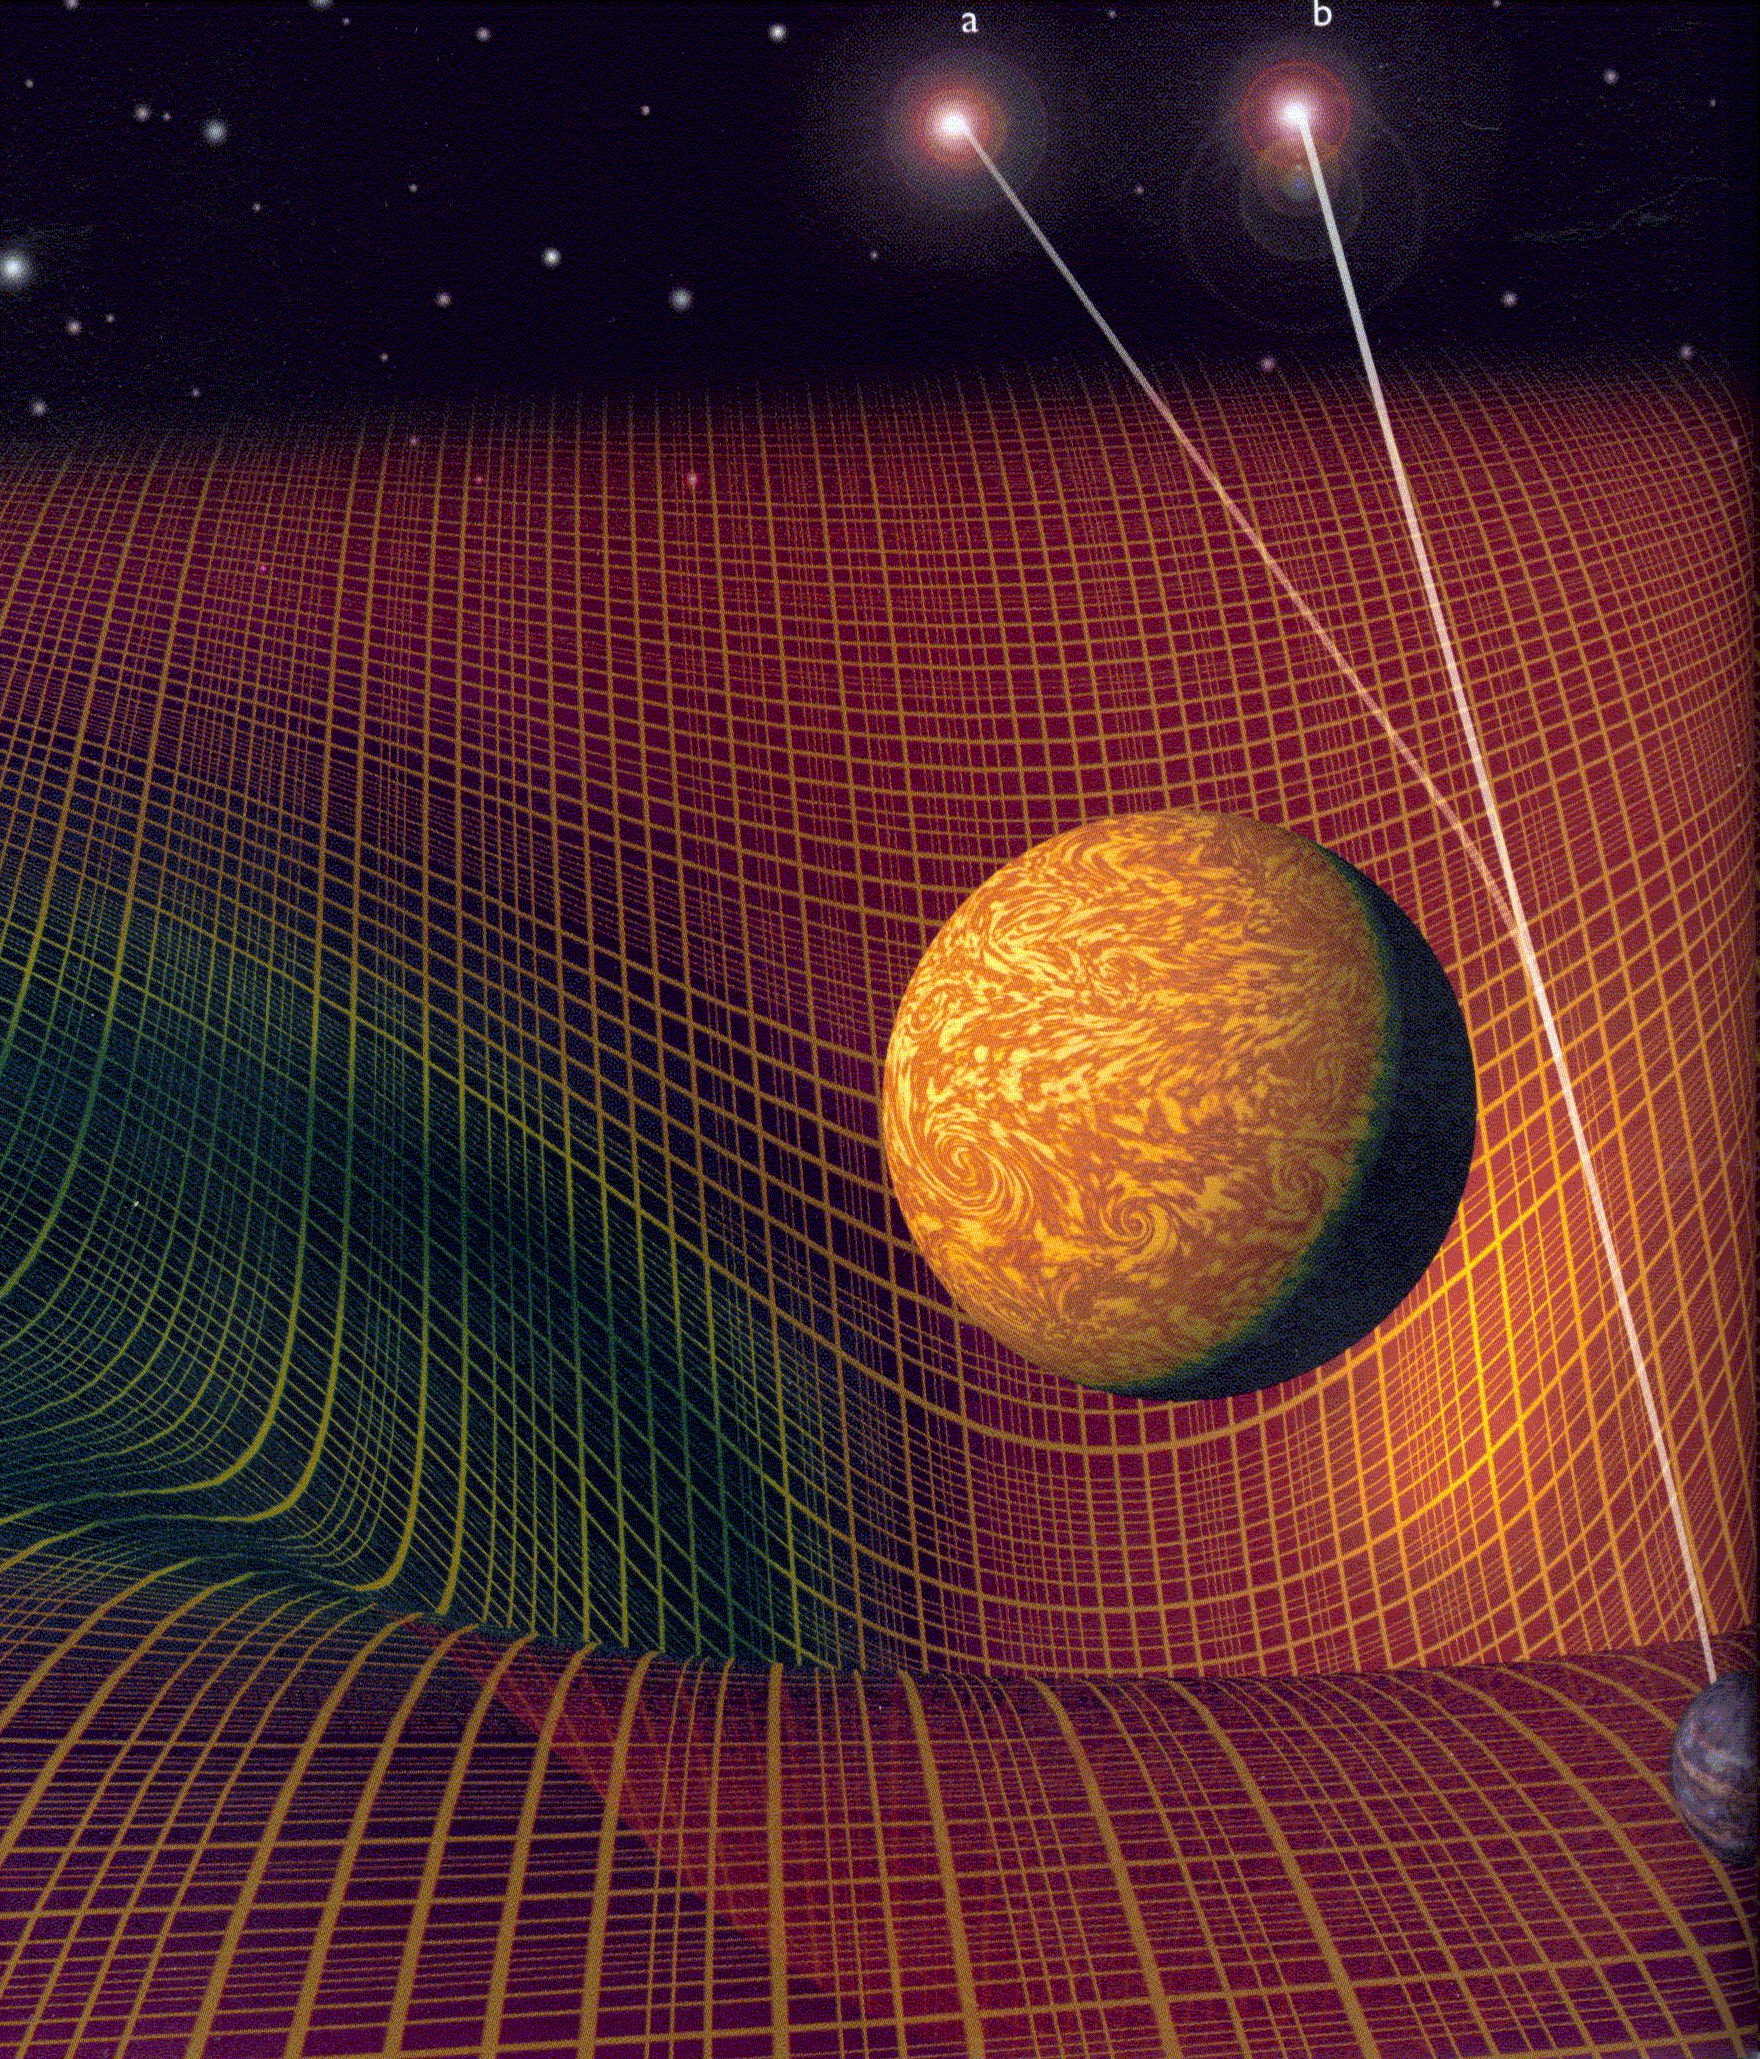
\includegraphics[width=0.5\columnwidth]{figures/Spacetime.jpeg}
            \caption{Credits: Hyper-Mathematics - Uzayzaman / Spacetime}
            \vspace{-0.5em}
          \end{figure}
        \end{block}
        \vspace{1ex}
        \begin{block}{Binary Lens with Orbital Motion\hfill \planeticon{earth}}
          Usually, in microlensing events static binary systems are taken into
          account, but binary systems do rotate

          The parameters to be determined using a fit in microlensing events by
          binary lens with orbital motion are
          \begin{itemize}
          \item Paczyński curve parameters: \(t_{0} \quad u_{0} \quad
            t_{\textup{E}} \quad \theta\)
          \item finite source effects: \(\rho_{\star}\)
          \item binary lens: \(b \quad q\)
          \item binary lens with orbital motion: \(a \quad e \quad i \quad
            \phi\)
          \end{itemize}
          In addition, with small mass ratios \(q\) there is the
          \alert{close-wide degeneracy} \(b \longleftrightarrow b^{-1}\)

          What if we knew the orbital period of the lenses
          \begin{equation*}
            P = 2\pi\sqrt{\frac{a^{3}}{GM}} =
            2\pi\sqrt{\frac{a^{3}}{Gm_{1}(1 + q)}}
          \end{equation*}
          \alert{independently}?
        \end{block}
        \vspace{1ex}
        \begin{block}{Fit to Real Data\hfill \planeticon{jupiter}}
          \begin{figure}
            \centering
            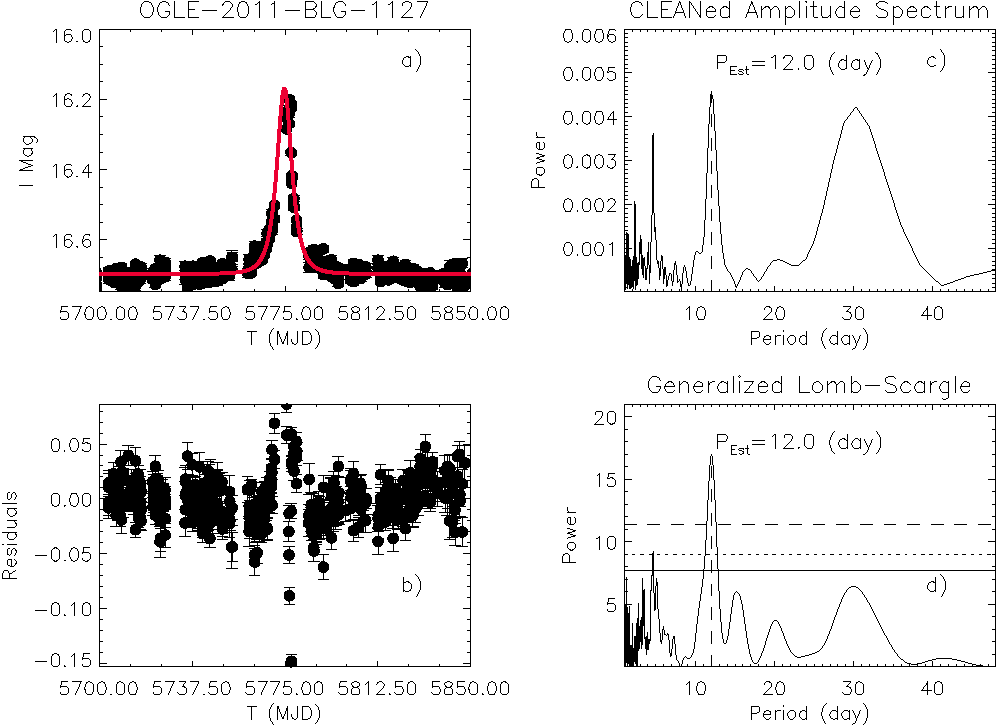
\includegraphics[width=0.7\textwidth]{figures/ogle322all}
            \caption{Event OGLE-2011-BLG-1127/MOA-2011-BLG-322}
            \vspace{-0.5em}
          \end{figure}
        \end{block}
        \vspace{1ex}
        \begin{block}{Conclusions\hfill \planeticon{saturn}}
          \begin{itemize}
          \item[\advice] Orbital period of the lenses should be \alert{shorter}
            than the Einstein time of the event or we must have a \alert{long
              observational window}
          \item[\advice] We fit the observed amplification curve to a \alert{simple
              Paczyński curve}, with four easily-guessable free parameters, and
            then perform a periodogram on the residue curve: the period so
            obtained is the \alert{period of the binary system}
          \item[\warning] We need to \alert{remove a very small region} around the
            maximum peak from the residue curve before performing the
            periodogram
          \item[\warning] Periodic feature with the same period far from the peak
            \(\implies\) \alert{source periodicity} (binary system, intrinsic
            variable, etc\dots)
          \end{itemize}
        \end{block}
      \end{minipage}
    \end{column}

    %%% Right column
    \begin{column}{0.44\textwidth}
      \begin{minipage}[T]{\columnwidth}
        \begin{block}{Detecting Exoplanets with Microlensing\hfill
            \planeticon{venus}}
          \alert{Microlensing} is a powerful tool to detect exoplanets: a binary
          system (lensing star with a companion planet) induces non-negligible
          deviations to the usual symmetric \alert{Paczyński light curve}
          \begin{figure}
            \centering
            % http://www.nature.com/nature/journal/v439/n7075/fig_tab/439400a_F2.html
            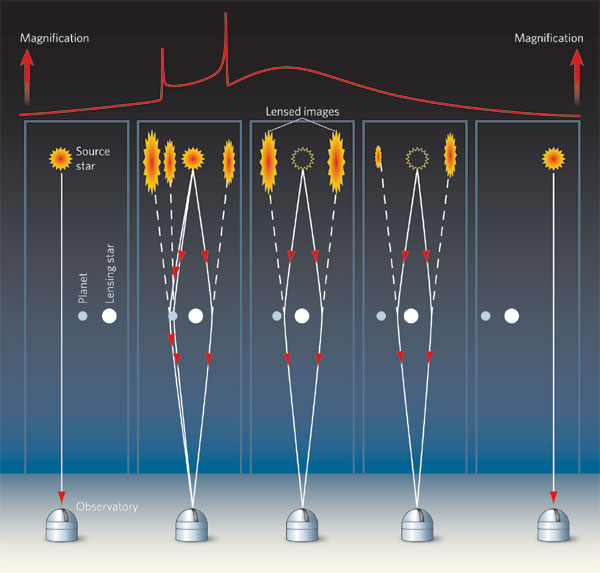
\includegraphics[width=.615\columnwidth]{figures/microlensing.jpg}
            \caption{Credits: Didier Queloz, \emph{Nature} \textbf{439},
              400--401.  \doi{10.1038/439400a}}
            \vspace{-0.5em}
          \end{figure}
        \end{block}
        \vspace{1.7ex}
        \begin{block}{Simulation: Amplification Curve and Periodogram\hfill
            \planeticon{mars}}
          \begin{figure}
            \centering
            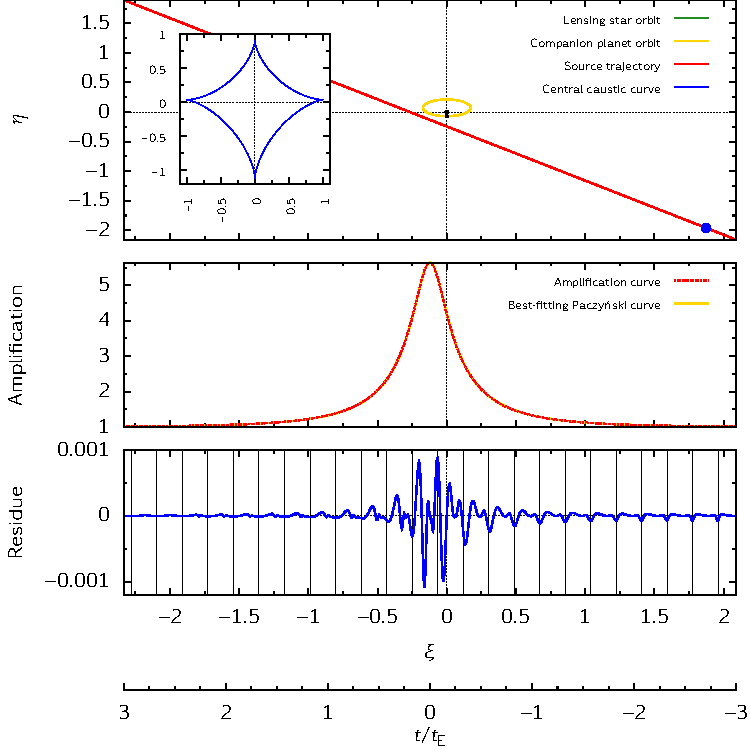
\includegraphics[width=0.775\columnwidth]{figures/figure2}\\[1.8ex]
            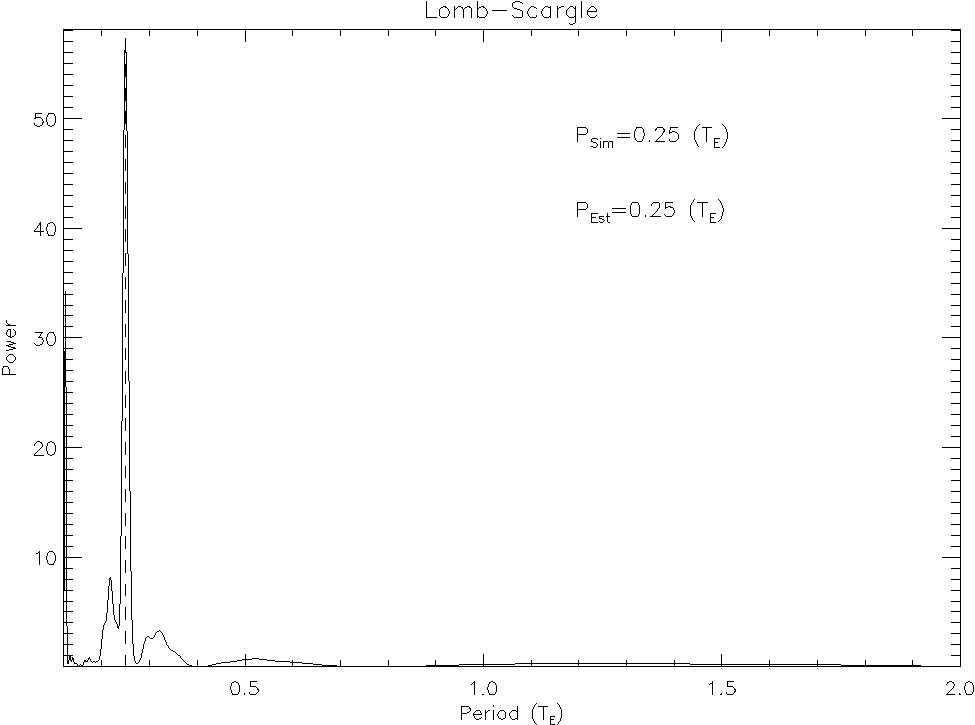
\includegraphics[width=0.775\columnwidth]{figures/lombscargle2}
            \caption{Parameters used: \(q = 10^{-3}\), \(a = 0.2\), \(e = 0.5\),
              \(i = \SI{45}{\degree}\), \(\phi = \SI{0}{\degree}\), \(P =
              t_{\textup{E}}/4\)}
            \vspace{-0.5em}
          \end{figure}
        \end{block}
        \vspace{1.7ex}
        \begin{block}{Reference\hfill \planeticon{uranus}}
          \begin{itemize}
          \item[{
\includegraphics[height=0.72em]{figures/beamericonarticle-crop.pdf}}]
            A. A. Nucita, M. Giordano, F. De Paolis, and
            G. Ingrosso. ``\emph{Signatures of rotating binaries in microlensing
              experiments}''. In: \emph{Monthly Notices of the Royal
              Astronomical Society} 438 (Mar. 2014), pp. 2466–2473.
            \doi{10.1093/mnras/stt2363} (scan here:~%
            \(\vcenter{\hbox{
\includegraphics[height=1em]{figures/paper}}}\)).
            \arxiv{1401.6288} (scan here:~%
            \(\vcenter{\hbox{
\includegraphics[height=1em]{figures/arxiv}}}\)).
          \end{itemize}
        \end{block}
      \end{minipage}
    \end{column}
  \end{columns}
\end{frame}
\end{document}

%%% Local Variables:
%%% mode: latex
%%% TeX-master: t
%%% ispell-local-dictionary: "british"
%%% End:
